
\section{Décalage de la Zone de Convergence}
Cette partie a fait l'objet d'un article, publié dans le journal Astronomy \& Astrophysics : \cite{cossou2013convergence}.

Le but de cette partie est de montrer que quand on met plusieurs planètes dans disque de gaz possédant une zone de convergence, ces dernières ne migrent pas individuellement mais au contraire se comportent comme un système ayant une migration globale. 

\subsection{Introduction}
Des planètes de l'ordre de quelques unités à quelques dizaines de masses terrestres interagissent avec le disque de gaz dans lequel elles se forment et génèrent des ondes de densité dans le disque \citep{goldreich1979excitation}. La planète elle même est influencée par cette onde de densité et migre par migration de Type I \citep{ward1997protoplanet}.

Dans les disques isothermes, la migration de Type I est gouvernée par le couple différentiel dû aux ondes de Lindblad. Pour les planètes, la migration qui en résulte est rapide et dirigée vers l'étoile centrale \citep{tanaka2002three}. Dans les disques radiatifs, un couple apparait dans la zone en fer-à-cheval de la planète. Ce dernier peut contrebalancer le couple différentiel de Lindblad au point de transformer la migration vers l'intérieur précédemment présentée en migration vers l'extérieur. Ainsi, dans de tels disques, la migration peut être dirigée soit vers l'intérieur soit vers l'extérieur \citep{paardekooper2006halting, kley2008migration}. Ceci rend possible l'existence de zone dans les disques où la migration est convergente. Ces dernières sont appelées zone de convergence \citep[CZs;][]{lyra2010orbital, paardekooper2011torque}.

\bigskip

À la zone de convergence, le couple de corotation (positif) compense exactement le couple différentiel de Lindblad (négatif). Ainsi, à la zone de convergence, une planète ne migre pas. Les zones de convergences pourraient ainsi concentrer les embryons planétaires et être le lieu de formation de planètes (ou cœeurs) massives \citep{lyra2010orbital, horn2012orbital}. 

Cependant, durant leur migration vers la zone de convergence les planètes vont interagir entre elles et se placer en résonance de moyen mouvement (Mean Motion Resonance : MMR), s'opposant ainsi à l'accrétion illimitée de matière à la zone de convergence \citep{morbidelli2008building, sandor2011formation}. Malgré cela, des collisions ont bien lieu à la zone de convergence quand les embryons sont emprisonnés dans une chaine de résonance avec suffisamment de corps pour engendrer des perturbations. De plus, la turbulence pourrait casser les résonances et augmenter le taux d'accrétion.

\bigskip

\cite{bitsch2010orbital} a montré que le couple de corotation était atténué quand une planète avait une excentricité telle que son orbite oscille sur une distance de l'ordre de la demi-largueur de la zone fer-à-cheval $x_s$. 

Quand deux planètes sont en résonance à cause de la migration convergente, leurs excentricités sont excités de manière continues malgré la présence du disque qui a tendance à amortir les excentricités et circulariser les orbites. \citep[par exemple ][]{cresswell2008three}. Ce phénomène devrait à son tour modifier le couple de corotation et ainsi modifier l'équilibre entre couple différentiel de Lindblad et couple de corotation. En conséquence, la migration de la planète elle-même devrait être modifiée.

\bigskip

Nous présentons des simulations de migration convergentes de planètes de faible masse ($M=1--10\unit{M_\oplus}$) dans un disque de gaz idéalisé (voir \refsec{sec:tanh_indep}). On utilise un modèle simplifié de rétroaction de l'excentricité sur le couple de corotation. Nous montrons que les planètes qui prisent de manière isolées migrent à la zone de convergence, ne migrent plus au même endroit quand il y a plusieurs planètes. Au lieu de ça, elles migrent à une position d'équilibre décalée vers l'intérieur du disque qui correspond à une somme nulle des couples exercées sur le système. 

La position de cet zone d'équilibre dépend de l'excentricité maintenue par perturbation mutuelle de chaque planète constituante du système.

\subsection{Méthode}
On modélise une Zone de Convergence (CZ : Convergence Zone) artificielle, qui imite une zone de convergence indépendante de la masse, c'est à dire que la position de la zone de convergence est la même pour toutes les planètes quelle que soit leur masse. En particulier, on s'intéresse à la zone de convergence que l'on peut trouver à une transition d'opacité telle que celle représentée sur \reffig{fig:shifted_CZ_torque_prof}, où l'on peut voir un renversement brutal du couple, qui passe de positif à négatif \citep[voir par exemple ][]{masset2011type}.

\begin{figure}[htb]
\centering
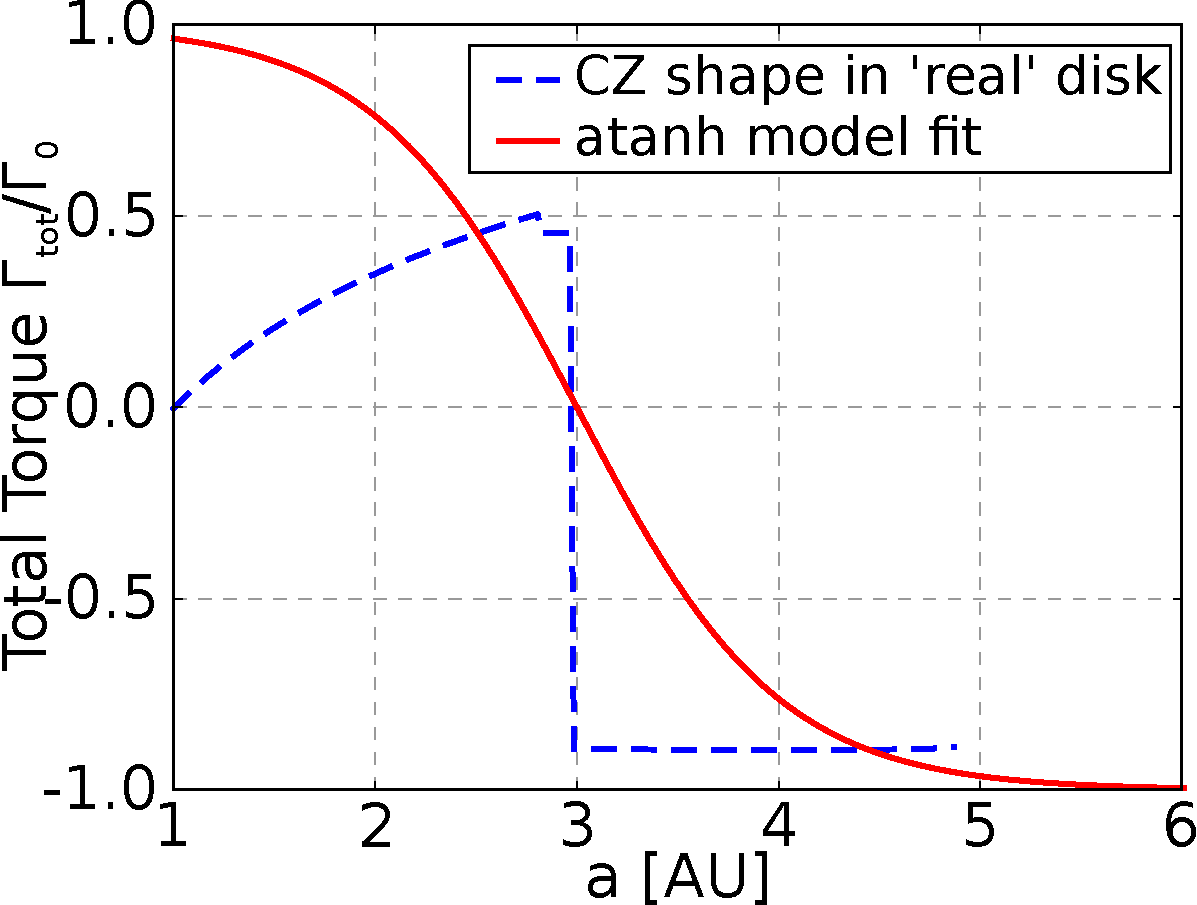
\includegraphics[width=0.49\linewidth]{figure/shifted/torque_zoom_CZ1.pdf}
\caption{Le couple total de notre disque standard est représenté en rouge. La ligne bleue pointillée représente le profil de couple ressenti par une planète de $10\unit{M_\oplus}$ autour d'une transition d'opacité, calculé à partir des équations de \cite{paardekooper2011torque}.}\label{fig:shifted_CZ_torque_prof}
\end{figure}

À noter qu'une fonction de Heavyside n'a pas été utilisée car la marche d'escalier dans le profil \textit{réel} n'est due qu'au fait que la table d'opacité n'a pas été lissée, on est donc témoin ici du changement de régime numérique, mais on ne s'attend pas à une transition aussi marquée dans un cas physique et non numérique.

La position de la zone de convergence était $3\unit{UA}$. À l'intérieur de $3\unit{UA}$, le couple est positif et égal à $\Gamma_0 = \left(\frac{q}{h}\right)^2\Sigma_p {r_p}^4 {\Omega_p}^2$., la migration se fait donc vers l'extérieur. Au delà de $3\unit{UA}$, le couple total est égal à $-\Gamma_0$. Ici $q$ est le rapport entre les masses de la planète et de l'étoile, $h$ est le raport d'aspect qui dépend du profil de température mais faut typiquement $0.05$. $\Sigma_p$, $r_p$ et $\Omega_p$ sont respectivement la densité de surface, la distance orbitale et la vitesse angulaire pour la planète. 

Le couple total est la somme du couple différentiel de Lindblad $\Gamma_L$ --- que l'on suppose constant et indépendant de $e$ --- et le couple de corotation $\Gamma_C$. Le principal intérêt de la zone de convergence artificielle est de s'affranchir de la forme très complexe du profil réel et ne garder que la zone de convergence, afin d'en étudier les effets de manière isolée.

\bigskip

\cite{bitsch2010orbital} montre que la structure de la zone fer-à-cheval est modiviée quand l'extentricité d'un corps massif augmente. En conséquence, son couple de corotation $\Gamma_C$, lié à cette région du disque, diminue. 

Nous avons élaboré une formule simple qui reproduit l'effet de l'excentricité sur $\Gamma_C$ par une simple calibration des simulations 3D de \cite{bitsch2010orbital} : 
\begin{align}
D &= \frac{\Gamma_C(e)}{\Gamma_C (e=0)} = 1 + a \cdot \left[\tanh(c) - \tanh\left(\frac{b * e}{x_s}+c\right)\right]\label{eq:eccentricity-influence}
\end{align}
où $x_s$ représente la demi-largeur de la région fer-à-cheval en unité de distance orbitale de la planète considérée, $e$ est l'excentricité de la planète, et notre ajustement statistique donne les valeurs suivantes pour les paramètres de la fonction :
\begin{align}
a &= 0.45 & b &= 3.46 & c &= -2.34
\end{align}

On défini $x_s$ comme \citep[voir][eq. 44]{paardekooper2010torque} :
\begin{align}
x_s &= \frac{1.1}{\gamma^{1/4}} \left(\frac{0.4}{b/h}\right)^{1/4} \sqrt{\frac{q}{h}}
\end{align}
où $\gamma$ est l'indice adiabatique, $q$ le rapport entre les masses de la planète et de l'étoile, $h$ le rapport d'aspect et $b/h$ la longueur de lissage du potentiel gravitationnel de la planète, afin d'éviter une divergence du potentiel au voisinage de la position de la planète (problème issu des simulations hydrodynamiques 2D qui se répercute sur les formules de \cite{paardekooper2011torque}).

\reffig{fig:shifted_CZ_D_profile} montre que notre formule simple \refeq{eq:eccentricity-influence} correspond bien à la tendance des simulations hydrodynamiques de l'effet de $e$ sur $\Gamma_C$, en particulier pour les excentricités faibles. Il faut tout de même noter qu'il y a peu de points \og expérimentaux\fg et qu'il semble y avoir des fluctuations aléatoires influençant les valeurs mesurées.

\begin{figure}[htb]
\centering
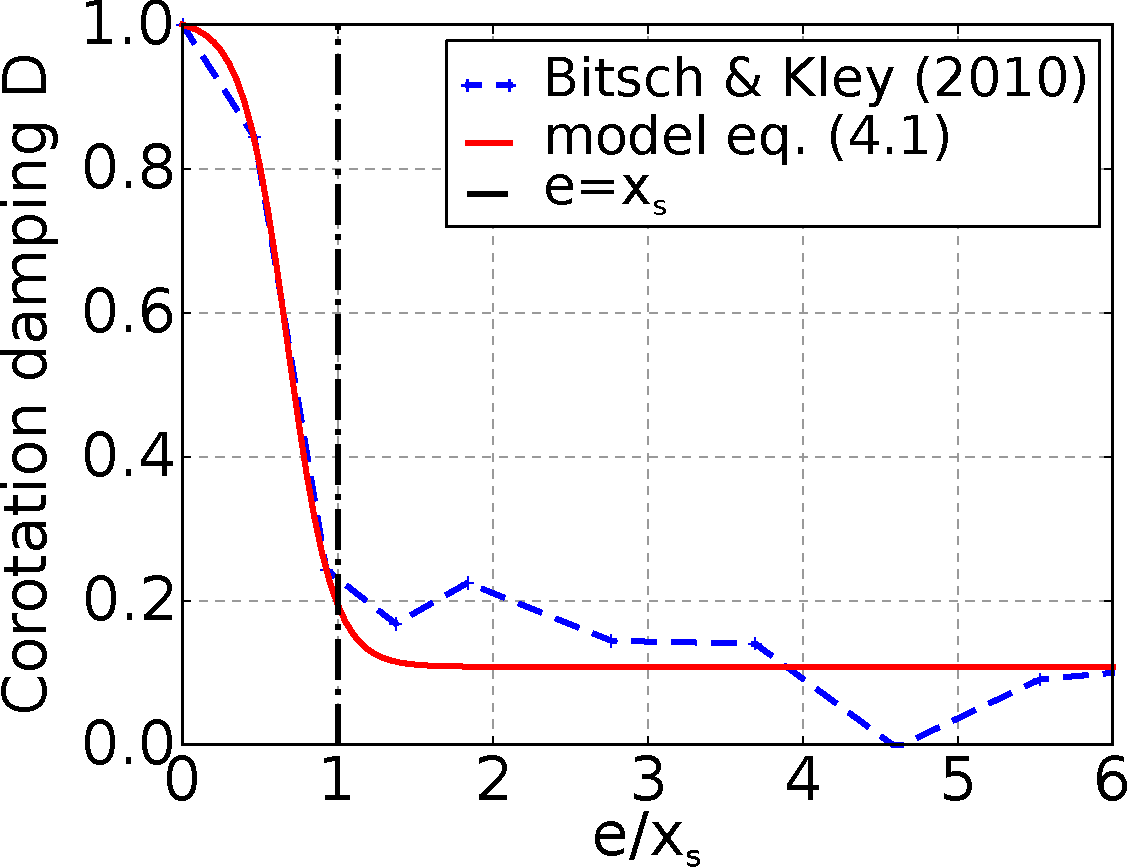
\includegraphics[width=0.49\linewidth]{figure/shifted/corotation_damping_profile.pdf}
\caption{Diminution du couple de corotation $\Gamma_C$ en fonction de l'excentricité $e$. On suppose que l'atténuation ($0<D<1$) du couple de corotation en fonction de l'extencité $e$ est la même dans un disque isotherme ou radiatif. Ainsi, on extrait la valeur de $D$ à partir de la figure 2 de \cite{bitsch2010orbital} en faisant la différence entre la valeur pour le disque radiatif et celle pour le disque isotherme, et normalisant de sorte que $D$ vale $1$ dans le cas $e=0$.}\label{fig:shifted_CZ_D_profile}
\end{figure}

\bigskip

Afin de réaliser nos simulations, nous avons utilisé une version modifiée de l'intégrateur \textbf{Mercury}\citep{chambers1999hybrid}. Nous avons inclu à la fois une zone de convergence artificielle (où $\Gamma = \Gamma_L+\Gamma_C$) et le fait que $\Gamma_C$ est modifiée par l'excentricité selon \refeq{eq:eccentricity-influence}. L'amortissement de l'excentricité et de l'inclinaison est modélisé via les formulées décrites dans \cite{cresswell2008three}. 

Nous supposons que le disque possède le profil de densité de surface suivant :
\begin{align}
\Sigma(R) = 500 \left(R/1\unit{AU}\right)^{-1/2} \unit{g.cm^{-2}}
\end{align}
Ce profil est alors utilisé dans le calcul de $\Gamma_0$ et de l'amortissement induit par le disque sur $e$ et $I$.

Pour implémenter la migration induite par le couple du disque $\Gamma$, on note que $\Gamma=\od{J}{t}$, et on défini une accélération de migration $a_m$ telle que\citep[eq. (14)]{cresswell2008three} :
\begin{align}
a_m &= - \frac{v}{t_m}
\end{align}
où $v$ est la vitesse de la planète et $t_m=J/\od{J}{t}$ le temps de migration ($J$ est le moment angulaire).

\bigskip

Dans toutes les simulations, les planètes était initialement sur des orbites à faible excentricité ($e<0.001$) et faible inclinaison ($I<1^\circ$). Chaque simulation a été intégrée pendant trois millions d'années, avec un pas de temps compris entre $0.4$ et $3$ jours.

\subsection{Le cas de deux planètes}
\reffig{fig:two-planets} montre l'évolution de deux planètes de $1\unit{M_\oplus}$ initialement de part et d'autre d'une zone de convergence située à $3\unit{UA}$. Alors qu'elles se rapprochent l'une de l'autre, les deux planètes croisent une série de résonances and finissent piégée dans la résonance \MMR{7}{6}. Les excentricités des deux planètes atteignent alors un équilibre entre excitation résonante et amortissement par le disque. Cette excentricité d'équilibre est environ égale à $0.5$ fois la demi-largeur de la zone fer-à-cheval $x_s$ et amorti le couple de corotation à environ $80\%$ de sa valeur nominale (quand $e=0$). 

\begin{figure}[htb]
\centering
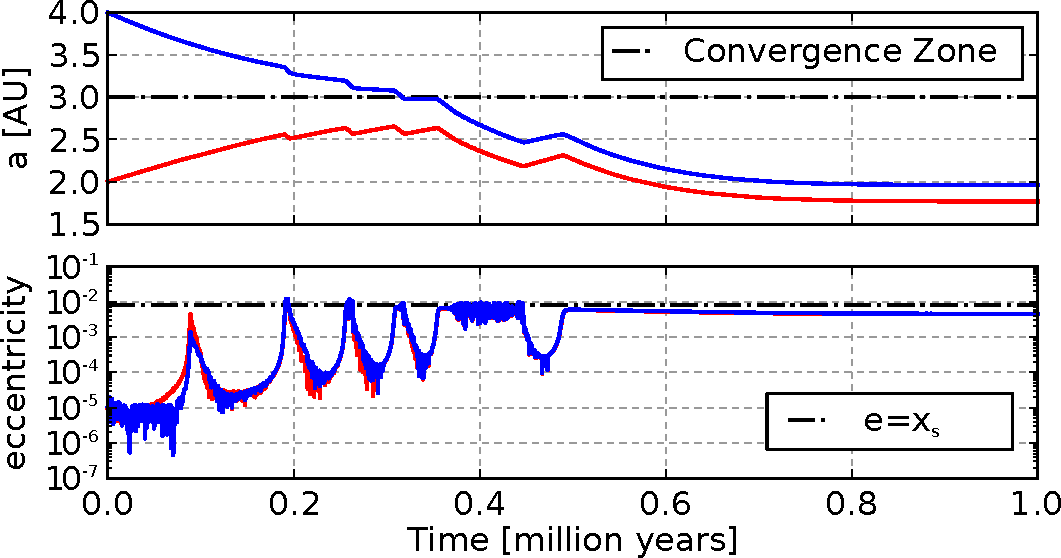
\includegraphics[width=\linewidth]{figure/shifted/corotation_damping_influence.pdf}
\caption{Simulation de la migration convergence de deux planètes de $1\unit{M_\oplus}$ vers la zone de convergence située à $3\unit{UA}$, la rétroactio de l'excentricité $e$ sur le couple de corotation $\Gamma_C$ étant incluse (voir Figure~\ref{fig:shifted_CZ_D_profile}).}
\label{fig:two-planets}
\end{figure}

Les planètes se stabilisent et arrêtent de migrer à $1.77$ et $1.96\unit{UA}$, toutes les deux à l'intérieur de la position nominale de la zone de convergence qu'elle ressentiraient si elles étaient seules et isolées dans le disque. Compte tenu de leurs excentricités, la zone de convergence de la planète la plus interne est décalée à $1.95\unit{UA}$ tandis qu'elle est décalée à $1.74\unit{UA}$ pour la planète externe (située à $1.96\unit{UA}$). On constate alors qu'aucune des deux planètes n'est à une position d'équilibre. Elles continuent de migrer chacune vers une position d'équilibre qui leur est inaccessible à cause de la présence de l'autre planète. 

Le décalage de la zone d'équilibre provient ici de l'équilibre nouveau entre le couple de Lindblad resté inchangé et le couple de corotation atténué par l'excentricité. \emph{Les deux planètes se stabilisent autour d'une zone où le couple total exercé sur le système dans sa globalité est nul, même si chaque planète prise séparément ressent un couple de migration non nul}. Aucune des deux planètes n'est ici à une zone de convergence (même celle calculée en tenant compte de l'atténuation du couple de corotation). 

Il est clair que les excentricités des planètes --- excitées par les interactions entre planètes --- sont le facteur clé pour déterminer la force du couple de corotation et la position effective de la zone de stabilisation du système. Pour deux planètes de même masse, le même comportement qualitatif est observé, quelle que soit la masse ou la résonance considérée : Une plus grande excentricité implique un amortissement plus fort du couple de corotation $\Gamma_C$ et une stabilisation du système de plus en plus proche de leur étoile. 

\subsection{Effet du rapport de masse}
Nous étudions maintenant le cas de deux planètes de masses différentes. \reffig{fig:mass_ratio_final_pos} représente les positions finales d'une série de simulations simples dans lesquelles une planète de $10\unit{M_\oplus}$ est placée systématiquement à $3\unit{UA}$ en compagnie d'une autre planète, placée à $4\unit{UA}$ et dont la masse varie successivement entre $0.1$ et $3\unit{M_\oplus}$. 

\begin{figure}[htb]
\centering
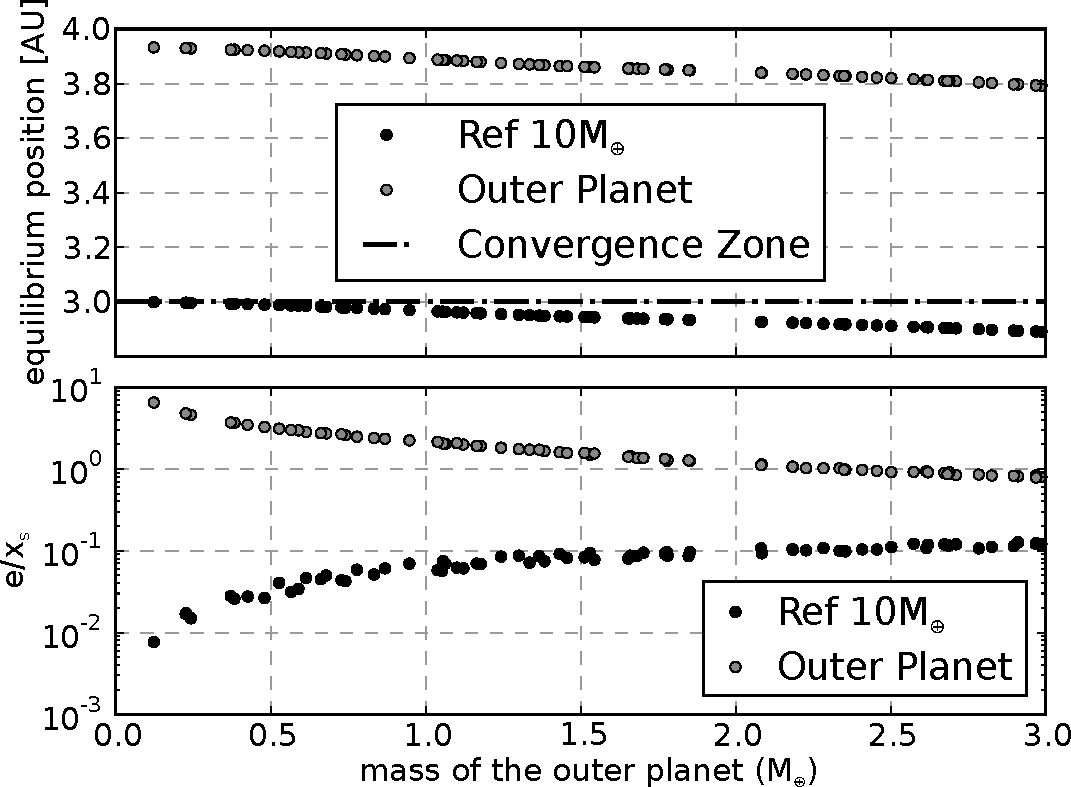
\includegraphics[width=0.95\linewidth]{figure/shifted/mass_ratio_influence.pdf}
\caption{Système final d'une série de simulations avec initialement une première planète à $3\unit{UA}$ de $10\unit{M_\oplus}$ et une deuxième planète à $4\unit{UA}$ dont la masse varie de $0.1$ à $3\unit{M_\oplus}$. Les graphiques montrent la position d'équilibre des planètes (en haut) et les excentricités normalisées par rapport à la demi-largeur de la zone fer-à-cheval $e/x_s$ (en bas) en fonction de la masse de la deuxième planète.}\label{fig:mass_ratio_final_pos}
\end{figure}

\bigskip

Dans \reffig{fig:mass_ratio_final_pos}, la planète externe est systématiquement en résonance \MMR{3}{2} avec la planète interne. Ainsi, la position finale des planètes est déterminée par leur masse respective ou, pour cette expérience, par la masse de la planète externe vu que la masse de la planète interne est fixe. 

Plus la deuxième planète est massive, et plus le décalage du système planétaire par rapport à la zone de convergence est important. En effet, une planète externe plus massive induit une excentricité plus importante pour la planète interne, ce qui correspond à un amortissement plus important de son couple de corotation $\Gamma_C$ et un décalage plus important de la zone d'équilibre du système. Compte tenu du fait que chaque planète possède une masse et une excentricité différentes, elles ressentent une zone de convergence différente (une pour chaque valeur de $e/x_s$). Pour autant, l'importance du décalage vers l'étoile centrale de la position d'équilibre est principalement déterminée par la dynamique de la planète la plus massive et de sa nouvelle zone de convergence.

\bigskip

\reffig{fig:mass_ratio_final_pos} représente uniquement un sous-ensemble de toutes les simulations de cette expérience. Pour des masses plus importantes, les deux planètes étaient dans des résonances différentes, ce qui causait des discontinuités dans le diagramme, rendant difficile sa lecture. Malgré tout, le comportement du système de deux planètes est qualitativement le même.


%TODO 
\section{Formation des super terre chaude}
%TODO 
%Observations : contraintes en fonction de la masse des planètes, séparation (en delta, et en p2/p1)
%
%autres modèles : 
%-in-situ (murray & hansens, ou chiang & laughlin, raymond 2008) il y a un résumé de tous les modèles dans raymond 2008
%-type I migraiton (terquem & papaloizou)
%
%_______
%environ une ou deux page pour cette intro


\section{Effets des paramètres du disque}
%TODO 
\subsection{Viscosité du disque}
%TODO 
\subsection{Profil de densité de surface}
%TODO 
\subsection{Profil de température}
%TODO 
\subsection{Masse du disque}
%TODO 
\subsection{Table d'opacité}
%TODO 